\newpage

\section*{Part C: Implementing SVM Variation [20 points] (Yichong and Prakhar) }
\textbf{Please attach your code as appendix to this problem.}\\
In the last homework, we derived a variant of SVM that explicitly maximizes the margin.
You can use any library on quadratic optimization (e.g., CVXOPT for python or \textsf{quadprog} for MATLAB) for this problem. Here is an instruction on CVXOPT.

Installation instructions of CVXOPT can be found \href{http://cvxopt.org/install/index.html}{here}. CVXOPT provides an easy interface for quadratic programming: The function \textsf{qp(P, q[, G, h[, A, b]])} solves the optimization problem
\begin{align*}
\text{minimize}_{x \in \mathbb{R}^n}\;  & (1/2) x^TPx+q^Tx \\
\text{subject to } & Gx \preceq h \\
& Ax=b
\end{align*}
for $P\in \mathbb{R}^{n\times n}, q\in \mathbb{R}^n, G\in \mathbb{R}^{m_1\times n}, h \in \mathbb{R}^{m_1}, A \in \mathbb{R}^{m_2\times n}, b \in \mathbb{R}^{m_2}$.
Here $\preceq$ means pointwise less than or equal; i.e., if $a \preceq b $ for $a,b \in \mathbb{R}^n$, then $a_i\leq b_i \forall i=1,2,...,n$, where the subscript indicates coordinates. Look into \href{http://cvxopt.org/examples/tutorial/qp.html}{here} for a concrete example including all details.

In last homework we want to solve the following primal problem:
\begin{align}
\min_{\boldsymbol{w}, \boldsymbol{\xi}, \rho}&\quad \frac{1}{2} {\boldsymbol{||w||}}_2^2 + \frac{1}{2}b^2- \rho + \frac{\lambda}{2} \sum_{i=1}^n \xi_i^2\label{eqn:primal}\\
\text{subject to} &\quad y_i(w^T \boldsymbol{x_i} + b) \ge \rho - \xi_i,\quad i = 1,\dotsc,n 	\nonumber
\end{align}


We derived a dual program of (\ref{eqn:primal}) in homework 2. (Have a look at the solutions if you did not solve it - we will release it soon.) Implement the dual program using CVXOPT. Compute results for both $\lambda=1$ and $\lambda=10$. The data is a toy dataset *train\_data.csv* in {\color{red}csv} format of size $\mathbb{R}^{100\times 2}$, and the training label is contained in the file *train\_label.csv* of size $\mathbb{R}^{100\times 1}$. Be careful that CVXOPT uses a slightly different matrix format than numpy; so either create your matrix in CVXOPT format, or use a numpy array and convert it into CVXOPT format using \textsf{A = cvxopt.matrix(A)}. \\
\textbf{Answer:}\\
From last homework, we know the dual form of this variant SVM as below:
$$\argmin_{\vec{\alpha}}\frac{1}{2}||\sum_{i=1}^{n}\alpha_iy_i\vec{x}_i||_2^2 + \frac{1}{2}(\sum_{i=1}^{n}\alpha_iy_i)^2 + \frac{1}{2\lambda}\sum_{i=1}^{n}\alpha_i^2 $$
s.t.
$$\sum_{i=1}^{n}\alpha_i=1$$
$$\alpha_i \geq 0$$
Therefore, we can use CVXOPT to solve this dual problem to get $\vec{\alpha}$:

Assume the data matrix and label matrix as below:
$$$$
\begin{equation}
\nonumber
\begin{array}{rcl}
X & = & [\vec{x}_1,\vec{x}_2,\dots,\vec{x}_n]^T \\
Y & = & \left[\begin{array}{cccc}
y_1 & 0 & \dots & 0 \\
0 & y_2 & \dots & 0 \\
\vdots & \vdots & \ddots & \vdots \\
0 & 0 & \dots & y_n
\end{array}\right]
\end{array}
\end{equation}

Then we can convert the dual form into the CVXOPT form using the following configuration:
\begin{equation}
\nonumber
\begin{array}{rcl}
P & = & Y^TXX^TY+\vec{y}\vec{y}^T+I/\lambda \\
\vec{q} & = & \vec{0} \\
G & = & -I \\
h & = & \vec{0} \\
A & = & [1,1,\dots,1] \\
b & = & 1 \\
\end{array}
\end{equation}

(a) \textbf{[4 points]} Suppose you use $\boldsymbol{\alpha}$ as the Lagrange multipliers in dual program. Given the dual solution $\boldsymbol{\alpha}$, compute the primal solution $\boldsymbol{w}, \boldsymbol{\xi}, \rho$ in terms of training data, $\lambda$ and $\boldsymbol{\alpha}$. (Hint: This has been computed in last homework, and you do not need to redo them.) \\
\textbf{Answer:}\\
From last homework, we know that:
\begin{equation}
\nonumber
\sum_{i=1}^{n}\alpha_i \vec{z}_i=\left[
\begin{array}{c}
\vec{w}^* \\
b^* \\
\sqrt{\lambda}\vec{\xi}
\end{array}\right],~~where~\vec{z}_{i}=\left[\begin{array}{c}
y_{i}\vec{x}_{i}\\
y_{i}\\
\frac{1}{\sqrt{\lambda}}\vec{e}_{i}
\end{array}\right]
\end{equation}
Therefore, 
\begin{equation}
\nonumber
\begin{array}{rcl}
\vec{w} & = & X^TY\vec{\alpha}\\
b & = & \vec{\alpha}^T\vec{y}\\
\vec{\xi} & = & \vec{\alpha}\frac{1}{\lambda} \\
\end{array}
\end{equation}
For any $\alpha_i\neq0$, $y_i(\vec{w}^T\vec{x}_i+b)=\rho-\xi_i$ (complementary slackness); therefore, we can derive $\rho$ as below:
$$\rho = \min_i(y_i(\vec{w}^T\vec{x}_i+b)+\xi_i)$$

(b) \textbf{[8 points]} For each value of $\lambda$, draw a scatter plot of the data and plot the decision border  (where
the predicted class label changes) as well as the boundaries of the margin (the area in which
there is a nonzero penalty for predicting any label). Use different colors for margins and border. Also use different colors for positive ($y=1$) and negative ($y=-1$) samples.\\
\textbf{Answer:}\\
See Fig.\ref{fig:svm}
\begin{figure}[!h]
	\centering
	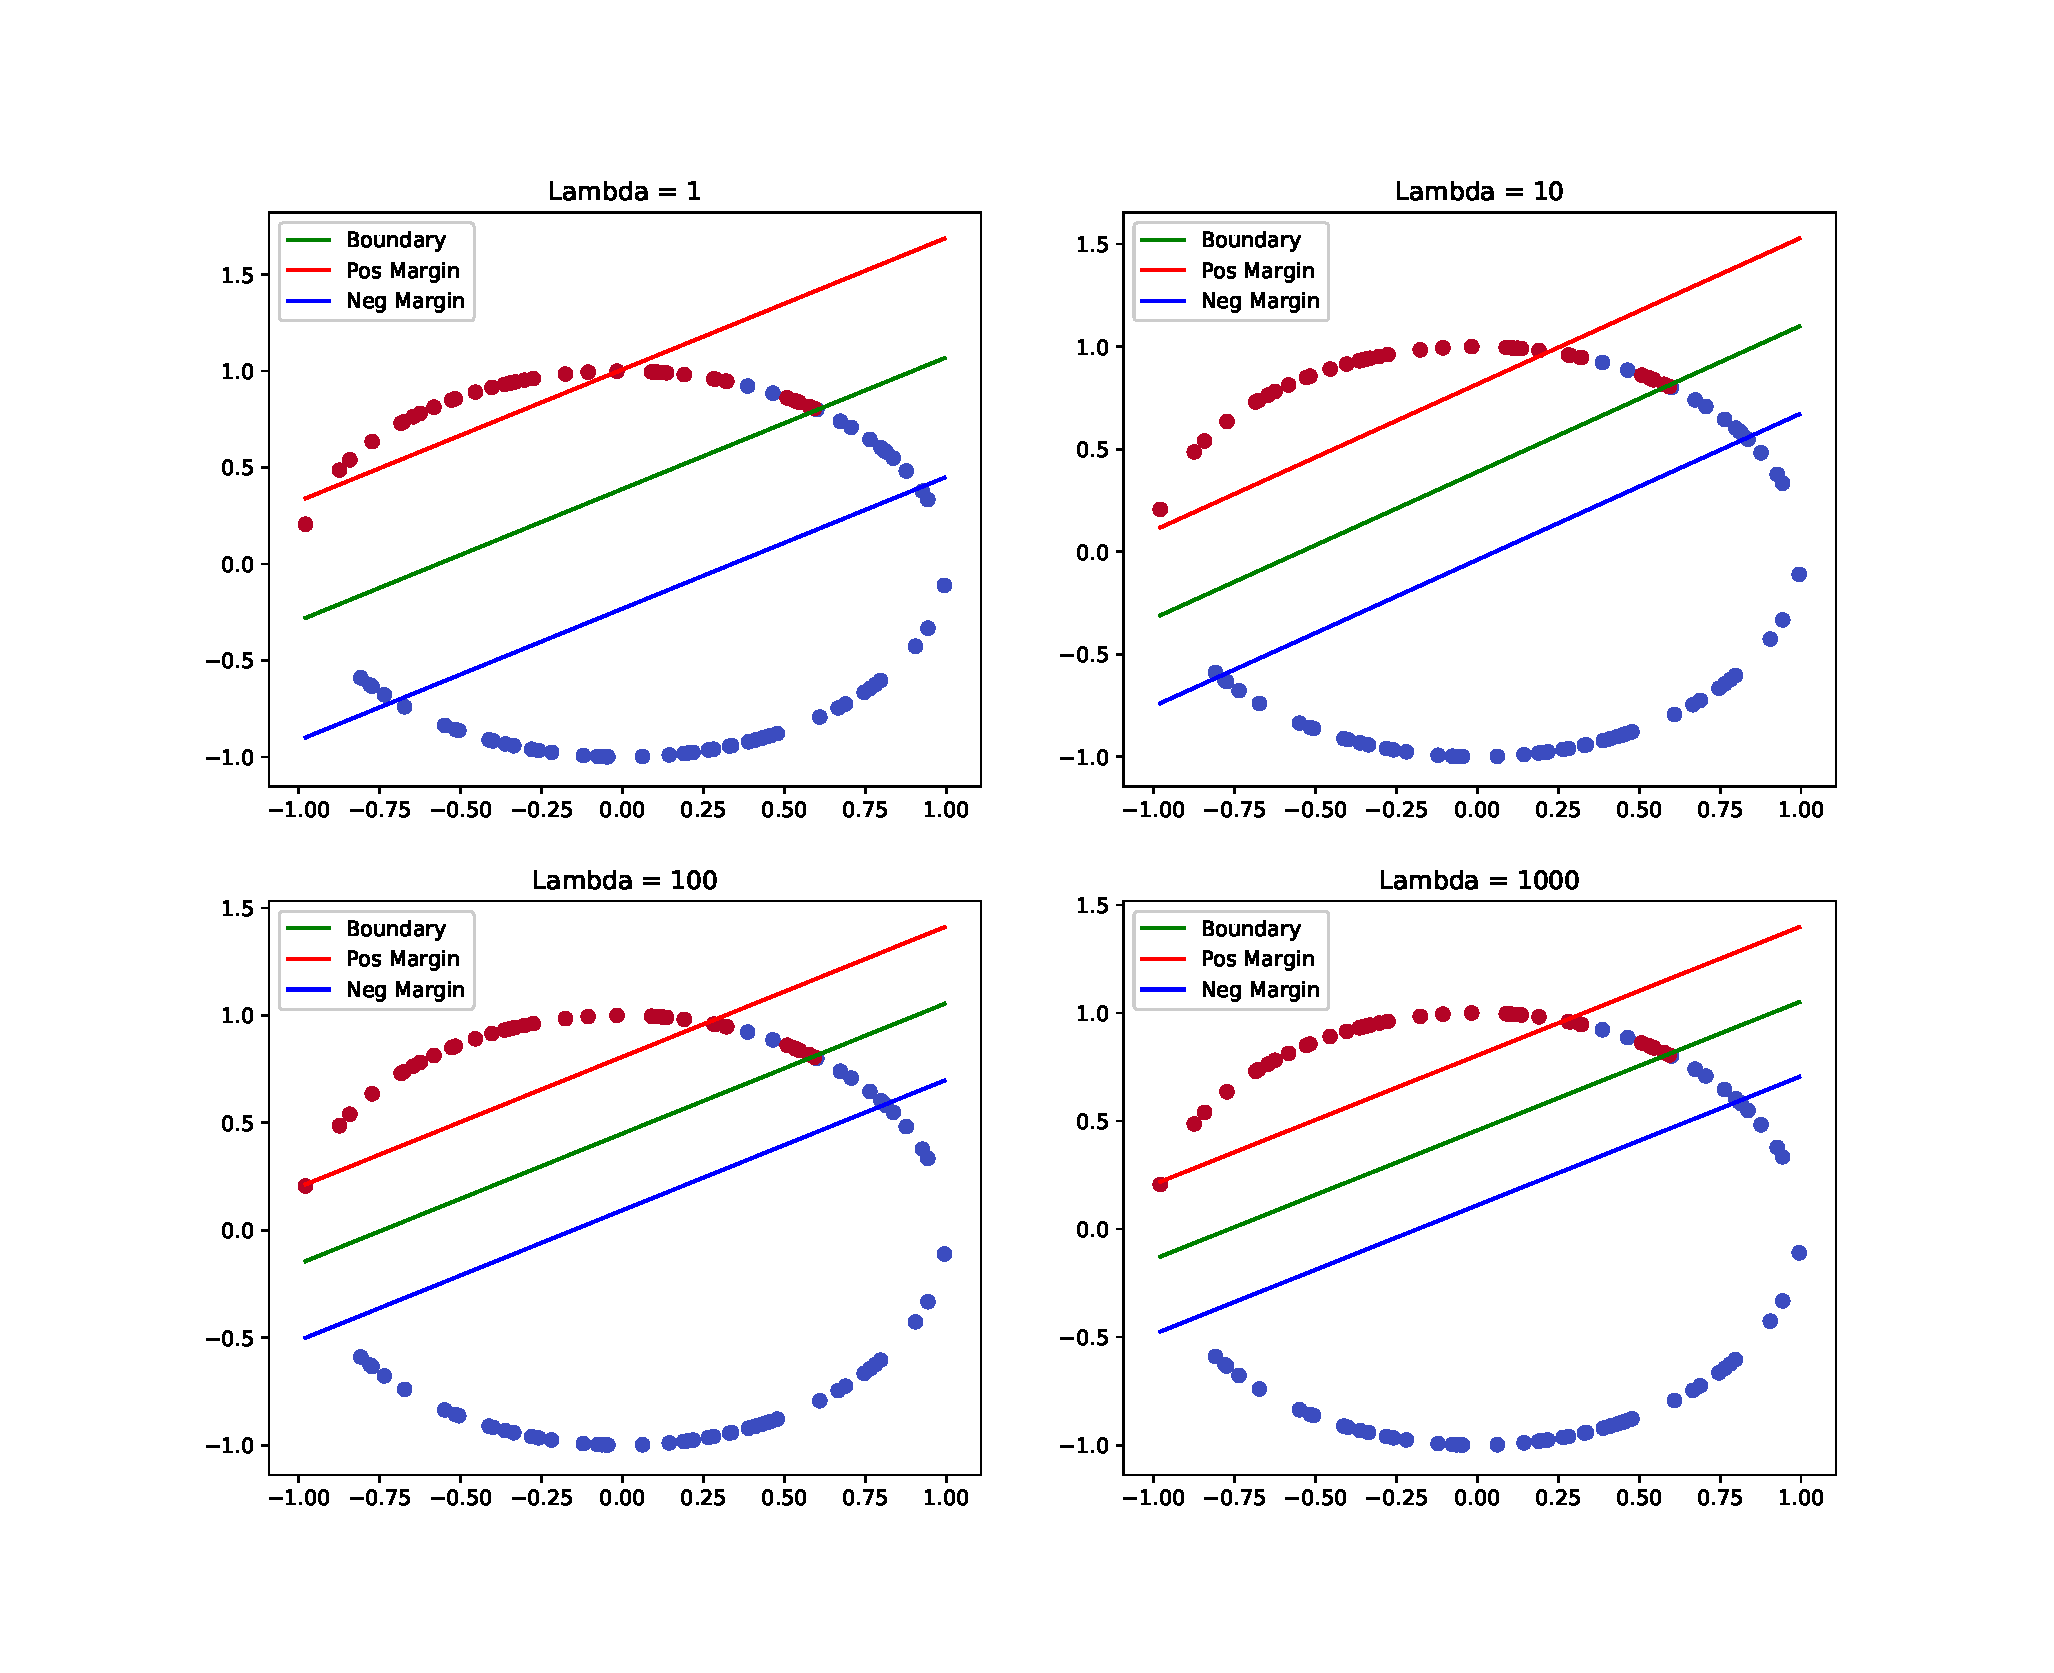
\includegraphics[width=0.8\textwidth]{./img/svm.eps}
	\caption{The Figure of Problem C.b}
	\label{fig:svm}
\end{figure}

(c) \textbf{[4 points]} Report the test error on the test set *test\_data.csv* and *test\_label.csv* for each value of $\lambda$.\\
\textbf{Answer:}\\
\begin{itemize}
	\item $\lambda = 1$: 0.15
	\item $\lambda = 10$: 0.13
	\item $\lambda = 100$: 0.15
	\item $\lambda = 1000$: 0.15
\end{itemize}

(d) \textbf{[4 points]} What is the difference between the result obtained in $\lambda=1$ and $\lambda=10$? Why is that?
\textbf{Answer:}\\
From the figure, we know that the margin area shrinks as the $\lambda$ increases, because higher $\lambda$ will less tolerate the slackness and thus shrink the margin area to remove more points from it. The test error of the SVM with $\lambda=10$ is lower than that with $\lambda=1$; however, this decreasing trend does not hold for the SVMs with $\lambda = 100$ and $\lambda = 1000$.

\newpage

\subsection*{Appendix: Code}


\lstinputlisting[language=Python]{./Python/hw3.py}